\newpage
\chapter{GİRİŞ}\label{ch:giris}

% GİRİŞ
Astrofiziksel nötrinolar hem nötrinoların temel özelliklerini hem de çekirdek-çökmeli süpernovalar (ÇÇSN) gibi astrofiziksel fenomenleri anlamamızı sağlayan, bilinen en hafif atom altı parçacıklardır \cite{Janka:2006fh, Janka:2012wk, Burrows:2012ew}. Laboratuvar ortamında nötrinoların özelliklerini belirlemeye çalışan deneyler olmasına rağmen, bu deneylerin çoğu sadece fiziksel niceliklerin üst sınırını belirler. Bu üst sınırlar, mesela nötrino manyetik momenti gibi, astrofiziksel olayların tüm fiziğini anlamak için yeterli değildir \cite{Brdar:2020quo, Super-Kamiokande:2020frs}. Bu nedenle astrofiziksel fenomenleri anlayabilmek için çok çeşitli nötrino çeşni (flavor) salınım simülasyonları yapılmalıdır.

% NÖTRİNO PARÇACIĞI
Standart model'de kütlesiz olarak öngörülen nötrinoların kütlesinin olduğu birçok deneyle ispatlanmıştır \cite{Gonzalez-Garcia:2007dlo,ParticleDataGroup:2018ovx}. Sadece zayıf etkileşimler sonucu ortaya çıkan nötrinoların çeşnisi beraber meydana geldiği lepton tarafından belirlenir. Zayıf etkileşimler sonucunda ortaya çıktığında çeşnisi belli olan nötrinolar boşlukta kütle özbazında (eigenbasis) ilerler. Bu da nötrinoların çeşnisinin salınımına sebep olur \cite{Super-Kamiokande:1998kpq, Maltoni:2004ei,LSND:2001aii,SNO:2002tuh, T2K:2017hed}. Bu durum en az bir nötrino kütle değerinin sıfırdan farklı olduğu durumda geçerlidir \cite{Giunti:2007ry}.

% NÖTRİNO ÇEŞNİ SALINIMI
Nötrino salınım fikrini 1950 yılında ilk olarak ortaya atan kişi Pontecorvo'dur \cite{Pontecorvo:1957cp}. Pontecorvo, laboratuvarda üretilen kaon adlı parçacığın antikaon'a salınmasından esinlenmiştir. Maki, Nakagawa ve Sakata, 1970 tarihinde yazdıkları makalede, nötrinoların antinötrinolara değil kendi çeşnileri arasında salınım yapabileceğini öne sürmüştür \cite{Maki:1962mu}. Evrendeki toplam çeşni sayısı, Standart Model'in öngörüsüne göre üçtür \cite{ParticleDataGroup:2018ovx} ve nötrino çeşnisi, tanımlanan bu üç kuantum büyüklük arasında salınır. Analitik hesaplar yapılırken üç seviyeli sistemler incelemek yerine iki seviyeli sistemlerin incelenmesi daha kullanışlıdır. Bu yaklaşıklık, hem hesap kolaylığı açısından önemlidir hem de kollektif çeşni evrimi gibi işlemci saati harcayan karmaşık sistemleri çözerken zaman kazandırır \cite{Duan:2010bg, Mirizzi:2015eza}. Bu tezin bazı noktalarında üç çeşnili evrim yapısına değinilecektir ancak elde ettiğimiz tüm hesaplar iki çeşni yaklaşıklığı ile yapılacaktır. Ayrıca nötrino salınım teorisi bilinen üç çeşniden daha fazla "çeşninin" varlığında da geçerlidir. Standart Model'de olmayan bu yeni çeşnili nötrinolara steril nötrinolar adı verilir. Bu tezde steril nötrino hesaplarına değinilmemiştir.

% SÜPERNOVA ORTAMI
1987 Yılında Büyük Macellan Bulutu içerisinde bir süpernova meydana gelmiştir ve bu astrofiziksel olay Dünya'dan gözlenmiştir. Gerçekleşen bu süpernova'ya SN1987A adı verilmiştir. O dönemde proton yarılanma süresi gibi fiziksel olayları incelemek için kullanılan deneyler, SN1987A optik gözlemlerinden birkaç saniye önce olağan dışı nötrino yoğunluğu gözlemlemişlerdir \cite{1987Natur.330..142S, 1987PhRvL..58.1490H}. Güneş nötrino gözlemlerini saymazsak, ilk defa kaynağı bilinen bir astrofiziksel fenomenden foton dışında bir parçacık gözlemlenmiştir.

SN1987A nötrino gözlemlerinin ardından süpernova fiziği araştırmaları hız kazanmış ve bu konuda sayısız araştırma yapılmıştır (\cite{Janka:2006fh} numaralı derlemeye ve bu derlemenin referanslarına bakınız.) Süpernova fiziği çok boyutlu, dinamik değişkenli ve başlangıç parametrelerine sıkı bağlı olduğundan dolayı simülasyonların gerçekleştirilmesi veya "patlatılması" epeyce zordur. Bunun için az da olsa deneysel veriye sahip olduğumuz SN1987A yapısını modelleyen sistemler kullanılmaktadır. Bu tezde geçen süpernova kelimesi ÇÇSN kelimesi yerine kullanılmıştır. ÇÇSN oluşumunun adımları kısaca şöyle özetlenir. Füzyon reaksiyonlar sonucu soğan yapısında olan Yıldız'ın çekirdeğinde demir/nikel bölgesi bulunmaktadır. Yüksek basınç ve sıcaklığa rağmen zincirleme füzyon reaksiyonu demir çekirdeğinde durur. Bunun sebebi demir/nikel çekirdeğinin aşırı stabil olmasıdır. Bu çekirdekler ile zincirleme füzyon reaksiyonu meydana gelmez. Başka bir dille ifade edersek, çekirdek başına düşen ortalama bağlanma enerjisi en yüksek çekirdek demirdir. Füzyon reaksiyonunun durduğu Yıldız'ın merkezinde, dışarıya doğru basınç kalmayınca içe doğru çöküş başlar (collapse.) Çöküşün başlamasının ardından Yıldız'ın merkezinde yaklaşık $ 10 $ km yarıçapında, biriken madde nükleer yoğunluğa erişir ve elektron dejenerasyon basıncı çöken maddenin daha fazla çökmesine izin vermez. Bu durumda çöken madde geri seker (bouncing.) Sekme sonucunda şok dalgası oluşur (shock formation) ve merkezden dışarı doğru madde aktarımı başlar. Ardından Yıldız'ın merkezinden çok büyük miktarda nötrino ve antinötrino açığa çıkar (neutrino burst.) Çok yüksek miktarda parlaklığa sahip olan nötrinolar Yıldız içerisinde biriken enerjinin yüzde $ 99 $'unu dışarıya taşır. Nötrinolar dışarı doğru giderken şok dalgasını "ısıtır" ve "iter" (neutrino heating.) Şok dalgası belli bir limit hıza eriştikten sonra patlama "gerçekleşti" denilir. Ardından açığa çıkan muazzam miktardaki nötrino Yıldız'ın içerisindeki enerjiyi dışarıya çıkartır (cooling.). Patlamanın başlangıcı sekmenin olduğu zaman dilimi olarak kabul edilir. Bu çalışmadaki nötrinoların kollektif çeşni evrimi ÇÇSN'nin soğuma evresinde incelenecektir. Soğuma evresi ise patlamanın başlangıcından yaklaşık bir saniye ile on saniye arasındaki dönemi kapsar. 

Süpernova sırasında Yıldız çekirdeğinde bulunan proto-nötron yıldızının manyetik alanı olabilir. Bu durumda süpernova simülasyonu yapılırken dinamik manyeto -hidrodinamik denklemler de çözülmelidir \cite{1970ApJ...161..541L, 2011ApJ...743...30T, Burrows:2012ew}. Çekirdeğin oluşturduğu manyetik alan, foto-ayrışma (photodissocciation) mekanizmasını etkileyerek şok dalgasının ilerlemesine ve ısınmasına yardımcı olur. Oluşan manyetik alan dinamik bir yapıya sahiptir ve zamana bağlı olarak değişmektedir. Bu tezde nötrino çeşni evrimi incelenirken bu manyetik alanın statik olduğu varsayılacaktır. Literatürde,statik manyetik alanın sabit değerde olduğu \cite{Abbar:2020ggq}, uzaklığın karesi ile ters orantılı olduğu \cite{Kharlanov:2020cti,deGouvea:2012hg, deGouvea:2013zp} ve uzaklığın üçüncü kuvveti ile ters orantılı \cite{Sasaki:2021bvu} olduğu yaklaşımlar bulunmaktadır. Bu tezde kullanılacak olan manyetik alan uzaklığın karesi ile ters orantılı olarak değişecektir.

% NÖTRİNO ELEKTROMANYETİK ETKİLEŞİM
Nötrinoların çeşni evrimi Yıldız içerisinde oluşan manyetik alandan etkilenmektedir \cite{Giunti:2014ixa}. Bu etkileşimin yapısı nötrinolar ile madde etkileşiminden farklı olarak gelecektir, çünkü nötrinolar yüksüz oldukları için foton ile etkileşmezler. Standart Model'in minimal bir genişlemesi yazıldığında, nötrino ile fotonu birinci mertebeden tedirgeme diyagramları ile etkileştirmek mümkündür \cite{Pal:1981rm}. Bu durumdan kaynaklı nötrinoların çok küçük değerli manyetik dipol momenti oluşacaktır. Standart Model'i, nötrino kütlesi kullanarak genişlettiğimizde nötrino manyetik momenti için elde edilen değer $ 10^{-19} $ Bohr magnetonu ($ \mu_{B} $) değerinden düşüktür \cite{Marciano:1977wx, Shrock:1982sc, Raffelt:1996wa, Bell:2005kz, Bell:2006wi}. Nötrino elektromanyetik etkileşimler nötrinonun doğasına bağlı olarak da farklılık gösterecektir. Eğer nötrinolar Dirac doğasında ise Standart Model'e göre nötrinolar sadece sol elli (left handed) olmalı, sağ elli anti-partneri olmalıdır. Dirac nötrinosunun deneylerle belirlenen manyetik dipol moment üst sınır değerleri \ref{fig:mu_nu} numaralı şekilde verilmiştir. Majorana nötrinolarında ise Dirac nötrinolarından elde edilen manyetik momentin sadece köşegen elemanları bulunacaktır. Hem Dirac doğası hem de Majorana doğasında nötrino manyetik momentinin tanımı model bağımlıdır. Bu tezde sadece Majorana nötrinoları dikkate alınmış olup nötrino manyetik momentinin $ \mu_{\nu}=5\times10^{-16} \mu_{B}$ değerinde olduğu kabul edilmiştir. Bu değer literatürde kullanılan ve deneylerden elde edilen büyüklüklerle uyumludur \cite{Bell:2006wi, Kuroda:2020pta, Super-Kamiokande:2020frs, Borexino:2017fbd, Brdar:2020quo}.

\begin{figure}[hbt!]
    \centering
    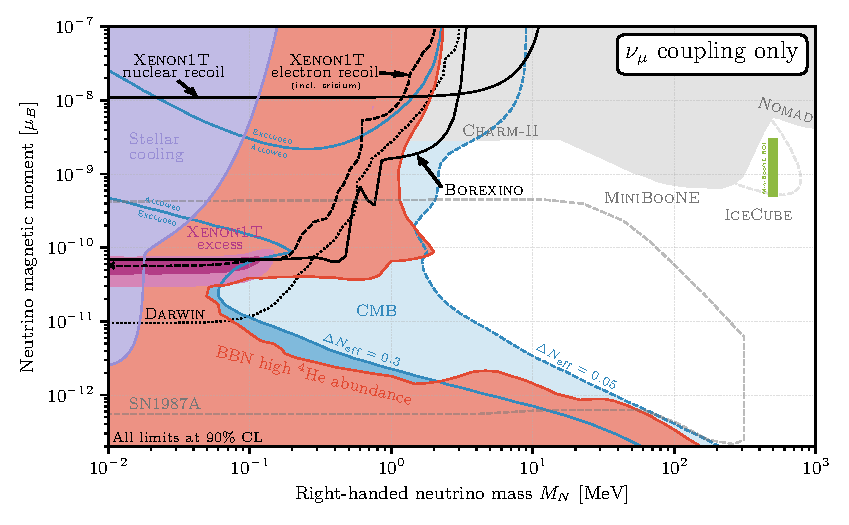
\includegraphics[width=\textwidth]{figures/Brdar_2020quo_mn_vs_munu_summary.pdf}
    \caption[Nötrino Manyetik Momentinin Üst Sınır Değerleri.]{Nötrino Manyetik Momentinin Üst Sınır Değerleri. Bu şekil \cite{Brdar:2020quo} numaralı kaynaktan alınmıştır.}
    \label{fig:mu_nu}
\end{figure}

% NÖTRİNO ÖZ KIRILIMI
ÇÇSN soğuma evresinde açığa çıkan nötrinolar hem cinsleri ile de etkileşecektir. Dikkate alınan test nötrinosu ÇÇSN ile açığa çıkan nötrino gazı ile etkileşime girecektir. Bu etkileşim terimleri yazılırken ortalama alan yaklaşıklığı kullanılmaktadır \cite{Sigl:1993ctk, Volpe:2015rla}. Nötrinoların bu tip etkileşimlerine nötrino öz-kırılımı (self-refraction) adı verilir. ÇÇSN'nın erken zamanında en önemli kollektif etki, nötrino öz-kırılımından gelir \cite{Duan:2006an, Duan:2008fd, Pehlivan:2011hp, Volpe:2013uxl}. Bu konu hakkında yapılan çalışmalar için \cite{Duan:2010bg} numaralı derleme makalesine bakınız.

% REZONANSLAR
Boşluktaki nötrino çeşni salınımlarında salınım genliği ve salınım frekansı değişmez. Nötrinoların çeşni evrimini etkileyen bir dış etki varsa, salınım frekansı ve genliği, o dış etkinin yapısına göre değişecektir. Eğer dış etki evrim sırasında değişmez kalırsa çeşni salınımlarının frekansı ve genliği de sabit kalacaktır. Bu dış etken nötrino-madde etkileşimi veya nötrino-manyetik alan etkileşimi olabilir.

Dış etkinin zamanla değişmesi durumunda ise çeşni salınım frekansı ve genliği değişimden etkilenecektir. Etkinin değişmesinden kaynaklanan salınım frekansı ile nötrino boşluk salınım frekansında bir uyum sağlanır ise çeşni salınımlarında ani bir değişim meydana gelecektir. Bu ani değişim sadece belli frekanslarda oluşur. Bu fenomene genel olarak \emph{rezonans} adı verilir. Bu özel frekansa ise \emph{rezonans frekansı} adı verilir. Rezonans fenomeni, doğal olarak salınım hareketi yapan sistemlere dış etki tarafından uygulandığında oluşabilir.

Madde içerisinde salınan nötrinoların rezonansa girebileceği ilk olarak Mikheev, Smirnov ve Wolfenstein tarafından bulunmuştur \cite{Wolfenstein:1977ue, Mikheyev:1985zog}. Bu fenomene de MSW rezonansı adı verilmiştir. Wolfenstein'ın madde içerisinde nötrino salınımları üzerine makalesinin yayınlamasının ardından Mikheev ve Smirnov Güneş içerisinde oluşan nötrinoların rezonansa girdiğini bulmuş ve literatürde solar nötrino problemi olarak adlandırılan sorun çözülmüştür. Bu çözüm Dünya'da yapılan deneylerle ispatlanmıştır \cite{Bellerive:2016byv}.

Nötrinoların madde içerisinden geçerken MSW rezonansına girmesi gibi manyetik alan içerisinden geçerken de salınımları rezonansa girebilir. Bu rezonansa SFP (spin-flavor precession) rezonansı adı verilir \cite{Okun:1986na, Fujikawa:1980yx, Cisneros:1970nq,Akhmedov:1988uk,Akhmedov:1987nc,Lim:1987tk}. SFP rezonansı nötrino manyetik momenti ve dış manyetik alan ile orantılıdır. Rezonansa girme koşulları büyük oranda MSW rezonansına benzemektedir. Bu rezonansın MSW rezonansından en büyük farkı nötrino-antinötrino geçişlerine olanak sağlamasıdır. 

% Bizim Yaptıklarımız
Bu tezde, nötrino-elektromanyetik etkileşimi varlığında elde ettiğimiz analitik sonuçları çeşni evrimini veren diferansiyel denklemin sayısal sonuçları ile karşılaştırıp bunların çoğunlukla uyumlu olduğunu ve uyumlu olması için gerekli şartların neler olduğunu gösterdik. Elde ettiğimiz şartlar dahilinde çeşni evrimini betimleyen yoğunluk operatörünün analitik ifadesini elde ettik. Bu analitik/sayısal karşılaştırmalarında öz-kırılım potansiyelini ihmal ettik, çünkü nötrino öz-kırılımı sistemi doğrusal olmayan hale getirmektedir. Karşılaştırmayı yaparken sayısal çözümlerdeki başlangıç koşullarını küçük oranda rastgele değiştirip kuantum fazlarından kaynaklanan farklılıkların açığa çıkmasını sağladık. Elde ettiğimiz analitik formülü bu fazlardan kaynaklanan değişimi kapsayacak şekilde yazdık. Analitik öngörümüz iki farklı rezonansın birbirinden ayrıldığı noktalarda geçerli olacaktır. Rezonansların birbirinden ne kadar ayrı olması gerektiğini nitel birkaç büyüklük tanımlayarak belirledik. Rezonansların birbirinden yeteri kadar ayrı olduğu durumlarda analitik öngörümüz sayısal sonuçlarımızla tutarlı sonuçlar vermektedir.

Bu tezin ikincil çıktıları ise şunlardır: Nötrino elektromanyetik etkileşimi ve nötrino madde etkileşimi varlığında yazılan hareket denklemini tedirgeme yöntemi kullanarak çözdük. Tedirgeme kuramından özvektörleri ve enerjiye gelen katkıları elde ettik. Buna ek olarak efektif iki çeşni yaklaşıklığı kullanıp sabit ve eksponansiyel manyetik alan için tam analitik çözümler elde ettik. Ayrıca gerçekçi ÇÇSN modeli için sayısal simülasyonlar yaptık. Bu simülasyonlarda nötrino öz-kırılımı ve ÇÇSN şok dalgası sisteme dahil edilmiştir. Son olarak PUSHing adlı parametrik ÇÇSN modeli kullanarak nötrinolardan kaynaklanan çekirdek sentezi ağ denklemlerini çözdük. Nötrino etkileşimlerinin ÇÇSN içerisinde nu-işlem elementlerininin bolluğunu arttırdığını belirledik.

% TEZİN İÇİNDEKİ BÖLÜMLER
Tezin planı şöyledir: İkinci bölümünde nötrino hareket denklemleri, boşluk salınımları ve dış ortamla etkileşimleri incelenmiştir. Nötrino evrimini betimleyen hareket denklemleri verildikten sonra boşluktaki çeşni salınımları için hareket denklemleri çözülmüştür. Madde ortamında çeşni salınımı yapan nötrinoların hareket denklemleri incelenmiş ve efektif açı yaklaşıklığı kullanılarak çözümler elde edilmiştir. Ardından elektromanyetik alan içerisinde hareket eden nötrinoların hareket dinamikleri belirlenmiş ve madde etkileşimi ile beraber alınarak hem tedirgenmiş çözümler hem de bazı profiller için analitik çözümler elde edilmiştir. Hareket kinematiğinin son bölümünde ise nötrino öz-kırılım potansiyeli elde edilmiştir.

Üçüncü bölümde ise nötrino çeşni salınımları sırasında meydana gelen rezonans durumlarına değinilmiştir. Landau-Zener (LZ) formülü kullanılarak geçiş olasılıklarının genel ifadeleri incelenmiş, ardından MSW ve SFP rezonanslarının gerçekleşme koşulları yazılmıştır. Rezonans bölgeleri evrimin adyabatikliğini belirlediği için adyabatisite parametresi de bu bölümde tanımlanmıştır.

Dördüncü bölümde ise bu çalışmamızın sonuçları olan simülasyonların analitik öngörüleri ve karşılaştırmalı sonuçları yer almaktadır. Yoğunluk operatörünün özbazdaki ifadesi analitik olarak bu bölümde elde edilmiştir. Ardından ÇÇSN içerisinde ilerleyen nötrinoların başlangıç koşulları ve geometrisi belirlenmiştir. Bu tezde elde ettiğimiz analitik/sayısal sonuç karşılaştırması oyuncak model alt başlığında yer almaktadır. Son olarak gerçekçi ÇÇSN modelinde nötrino etkileşimlerinin rolleri dört farklı etkileşim modeli kullanılarak incelenmiştir.

Beşinci bölümde ise nötrinoların süpernova içerisindeki çekirdek sentezlenmesine (nucleosynthesis) olan katkısı üzerine çalışmalar bulunmaktadır. Bu bölümde PUSHing adlı süpernova simülasyonu ve çekirdek sentezleme ağı kullanılarak Lityum ve Bor izotoplarının kütle kesirleri elde edilmiştir. Nötrino işleminin veya nötrino ile sentezlemenin (nu-process), bu izotopları sentezlemede önemi ortaya konmuştur.

Çalışmalarımızın sonuçları ve tartışması sonuç bölümünde incelenmiştir.

Çalışmamızda, hem kolay sayısal hesaplamalar yapmamıza olanak sağlayan matris notasyonu hem de operatör notasyonu kullanılmıştır. Ayrıca hesaplamalarda doğal birimler kullanılmıştır. Yani ışık hızı, Plank sabiti ve Stefan Boltzman sabiti $ 1 $ alınmıştır. Gerekli olduğu yerlerde uygun dönüşümler kullanılmıştır. Buna ek olarak nötrinoların hızı ışık hızına çok yakın olduğu için (erken evren soğuk nötrinolar dışında) zaman $ t $ ve konum $ r $ eşdeğer olarak görülmüştür. Bundan dolayı zamana bağlı olarak tanımlanan denklemler yerine konumla değişen denklemler yazılmıştır.